The diagram of the described compartment model is depicted on Figure \ref{fig:compartment}. \\


\begin{figure}[!h]
  \centering
  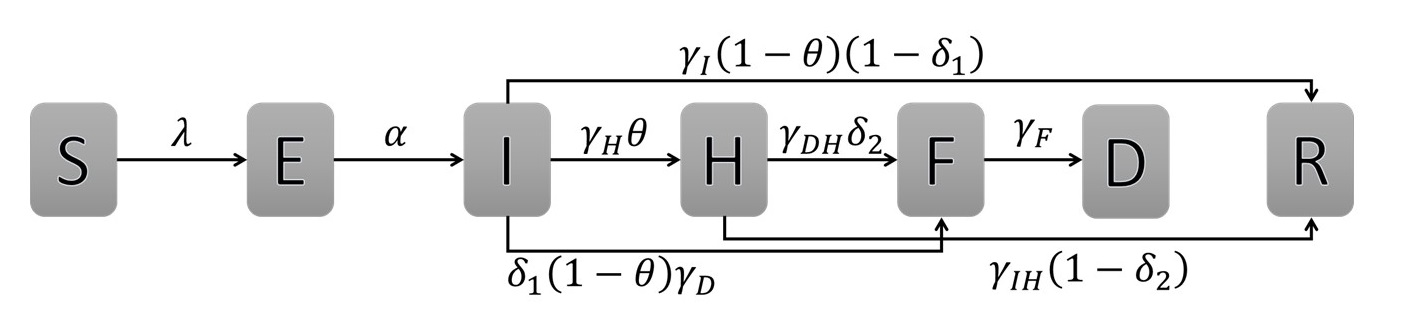
\includegraphics[width=0.7\textwidth]{compartment}
  \caption{Compartment Model of the Ebola Epidemic in Liberia  \newline  Being S: Susceptible, E: Exposed, I: Infectious, H: Hospitalized, F: Funeral,  R: Recovered and D: Dead. All the possible flows are specified by the arrows and the parameters that direct them. Note that $\lambda = \beta_{I}I+\beta_{H}H+\beta_{F}F $, being a combination of all the $\beta$ transmission terms shown in Table~\ref{tab:knownParameters} } 
\label{fig:compartment} 
\end{figure}


The governing equations of the system dynamics described above are the following:

\begin{eqnarray} 
\label{SDeqn}
\frac{dS}{dt} = - \frac{\beta_{I}SI+\beta_{H}SH+\beta_{F}SF}{N} \label{eqn:SD1}\\
\frac{dE}{dt} =  \frac{\beta_{I}SI+\beta_{H}SH+\beta_{F}SF}{N}-\gamma_P E         \label{eqn:SD2}\\
\frac{dI}{dt} =  \gamma_P E - [\gamma_{H}\theta + \gamma_{I}(1-\theta)(1-\delta_{1})+\gamma_{D}(1-\theta)\delta_{1}]I   \label{eqn:SD3}\\
\frac{dH}{dt} = \gamma_{H}\theta I - [\gamma_{HF}\delta_{2}+\gamma_{IH}(1-\delta_{2})]H \label{eqn:SD4}\\
\frac{dF}{dt} = \gamma_{D}(1-\theta) \delta_{1} I + \gamma_{DH}\delta_{2} H-\gamma_{F} F     \label{eqn:SD5}\\
\frac{dR}{dt} = \gamma_{I}(1-\theta)(1- \delta_{1}) I + \gamma_{HR}(1-\delta_{2}) H       \label{eqn:SD6}\\
\frac{dD}{dt} = \gamma_{F} F     \label{eqn:SD7}
\end{eqnarray}\\

where each of the parameters are defined on Tables ~\ref{tab:knownParameters} and ~\ref{tab:calibratedParameters}



%EQUATION DESCRIPTION
\noindent The equations described above come from a species balance, which guarantees that any individual is lost. $Accumulation = Input - Output$, in our case,

\begin{equation}
\frac{d (Accumulation)}{dt} = \frac{d (Input)}{dt} -\frac{d (Output)}{dt} \nonumber
\end{equation}


Equation \ref{eqn:SD1} describes the changes with respect to time on the Susceptible population, the transition from S to I depends on the product $\beta_{I}SI+\beta_{H}SH+\beta_{F}SF$, which specifies that such changes are given by the contact rate with the comparments I, H and F (all of them have Ebola), and the respective number of individuals on each compartment.\\

Equation \ref{eqn:SD2} describes the changes on the Exposed individuals. The number of individuals on this comparment depends on the number of individuals that become E, which depends on the same product as \ref{eqn:1}, substracting the number of individuals that transitions from E to I after the incubation period $\gamma_P$.\\

Equation \ref{eqn:SD3} describes the changes on the Infected patients, equally depends on the number of individuals that become I after the incubation period $\gamma_P$, substracting the individuals that transitions from I to H, which is given by the product between the transition rate from I to H and the probability a case becomes H; in the same way, substracting the individuals that transitions from I to R, given by  the product among the duration of infection rate, the probability a case is NOT hospitalized and the death rate of an unhospitalized case. Finally substracting the individuals that transitions from I to F , given by the product between the transition rate from Infected to Dead,  the probability a case is NOT hospitalized and the death rate of an unhospitalized case.\\

Equation \ref{eqn:SD4} describes the changes on the Hospitalized patients. It depends on the number of individuals that transitions from I to H, given by the  product between the transition rate from Infected to Hospitalized and the probability a case is Hospitalized;  substracting the individuals than transitions from H to D, given by the product among the transition rate from Hospitalized to Dead and the death rate of a hospitalized case, and finally, susbtracting the people that transitions from H to R, which is given by the product between the transition rate from I to R and the survival rate of an hospitalized case.\\

Equation \ref{eqn:SD5} describes the changes on the Funeralized compartment.  Depending on the number of individuals that transitions from I to D, which is given by the product between the transition rate from I to D, the probability a case is NOT hospitalized and the death rate of an unhospitalized case. Adding the people who transitions from H to F , which is given by the product between the transition rate from H to D and the death rate of an hospitalized case. Finally substracting the individuals who already have been buried.\\

Equation \ref{eqn:SD6} describes the changes on the Recovered compartment. Depending on the transition from I to R, which is given by the product between the duration of infection rate, the probability a case is NOT hospitalized and the survival rate of an Unhospitalized rate. Adding  the individuals who transitions from H to I, which is given by the product among the transition rate from I to H and the survival rate of a hospitalized case.\\

Equation \ref{eqn:SD7} describes the changes on the Funeralized compartment, which solely depends on the rate of duration of a traditional funeral.\\





%Parameter calibration
\subsection{Parameter Calibration}

The parameter values which represent biological process ($\alpha, \gamma_{I}, \gamma_{D}, \delta_{1}, \delta_{2}$) or social custom ($\gamma_{F}$) were discovered in many sources [reference], while the parameters which represent social behavior ($\mathcal{P}=\{\beta_{I}, \beta_{H}, \beta_{F}, \gamma_{H}, \theta\}$) are site-dependent and unknown (see Table and Equation for the detail of the parameters). $\gamma_{DH}$ and $\gamma_{IH}$ are also unknown, but we assume that they are dependent on other variables ($1/\gamma_{DH}$=$1/\gamma_{D}$-$1/\gamma_{H}$ and $1/\gamma_{IH}$=$1/\gamma_{I}$-$1/\gamma_{H}$). In this chapter, we calibrated $\mathcal{P}$ based on our systematic model (equation link) and the data of cumulative deaths in Liberia from March 2014 to July 2015 \cite{CDCData}.\\


\begin{figure}[!h]
  \centering
  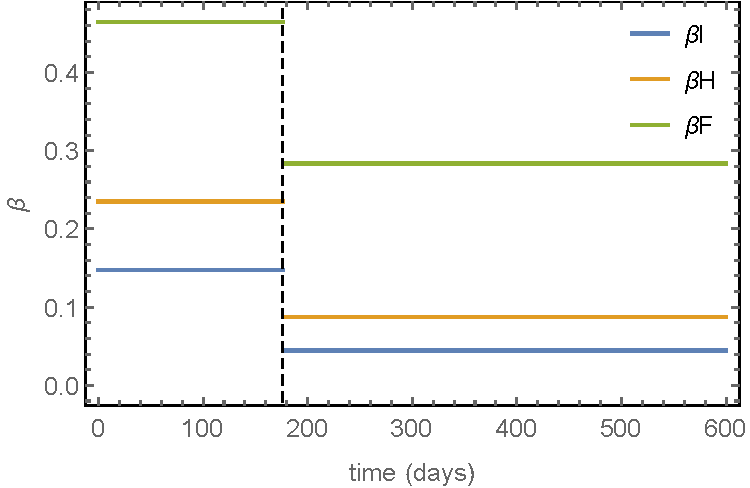
\includegraphics[width=0.7\textwidth]{BetaStepFunction.pdf}
  \caption{$\beta$ step function} 
\label{fig:BetaStepFunction} 
\end{figure}



\subsection{Bayesian calibration framework}

We use Bayesian methodology to calibrate our unknown system parameters. It is a versatile tool which is utilized in many calibrations of complicated systems owing to its merit that a little or no information on the parameter values is not an obstacle to use it. The calibration procedure starts from choosing a distribution in the space of parameters we concern. This distribution, which is called `prior distribution' ($\mathcal{D}_0$), can be a simple like uniform distribution or intuitively chosen parametric distribution. Based on the available data and mathematical setup, we evaluate the likelihood weight for the samples from $\mathcal{D}_0$ with which we update to the weighted distribution `posterior distribution' ($\mathcal{D}_1$) from $\mathcal{D}_0$. Multiple updates ($\mathcal{D}_1$ to $\mathcal{D}_2$, $\mathcal{D}_2$ to $\mathcal{D}_3$, ...) facilitate to get more straightforward pattern on the distribution.\\
To calibrate the unknown parameters ($\mathcal{P}$), we started from a uniform distribution in the range determined based on numerical exploration and previous researches (See Table \ref{tab: PriorRanges}) \cite{Rivers2014}. \\

\begin{table}[ht]
\caption{Range of the prior parameter space} % title of Table
\centering % used for centering table
\begin{tabular}{c c c c c}
\hline\hline %inserts double horizontal lines
$\beta_{I}$ & $\beta_{H}$ & $\beta_{F}$ & $\gamma_{H}$ & $\theta$ \\ [0.5ex]
\hline % inserts single horizontal line
$(0,0.5)$ & $(0,0.5)$ & $(0,1)$ & $(2,7)$ & $(0,0.5)$ \\ [0.5ex]
\hline
\end{tabular}
\label{tab:PriorRanges}
\end{table}


To each random choice ($\mathcal{P}_0$) from the prior distribution, we assign likelihood weight by comparing the real world data ($\mathcal{D}_R$) and data simulated with $\mathcal{P}_0$ ($\mathcal{D}_S$). Multiple choices of parameters and their weights will eventually construct the posterior distribution of $\mathcal{P}$. In this methodology, we provide multiple likely parameter sets, rather than a single best fit. Detailed description on the calibration procedure is:\\

Step 1) Choose a random $\mathcal{P}_0$ from the prior distribution

Step 2) Solve our deterministic system (equation link) with $\mathcal{P}_0$ and given initial value $\{S_0,E_0,I_0,F_0,D_0,R_0\}$, then evaluate $\mathcal{D}_S=\{D(t_i)\}$ for all dates $\{t_i\}$ corresponding to the cumulative death data ($\mathcal{D}_R$).

Step 3) Evaluate likelihood of $\mathcal{P}_0$: $Exp[-Norm(\mathcal{D}_R-\mathcal{D}_S)/Norm(\mathcal{D}_R)]$

\emph{Repeat Step 1-3 multiple times and make large number of {parameter + likelihood} ensembles. Generate posterior distribution with them.}

\subsubsection{Results and validation}
We applied our systematic model and calibration method for Ebola spread in Liberia 2014-2015. Two sets of cumulative mortality data (pre-intervention, post-intervention) are used to calibrate pre- and post-intervention parameter calibration, respectively. We assume that about a forth (1 million) of the total Liberia population (the 4.3 million [reference]) are involved in the transmission, and the rest are not in any chance due to geographical and behavior reason. For the calibration of before intervention parameters, we used the data for 176 days (March 2014 to September 2014), and initial value $\{S_0,E_0,I_0,F_0,D_0,R_0\}$=$\{10^6-1,0,1,0,0,0\}$ assuming that initial outbreak started from a single infected person in a million population. The calibration of intervention parameters is based on the data for 306 days (September 14 to July 15), and initial value $\{S[176],E[176],I[176],F[176],D[176],R[176]\}$ which are evaluated from calibrated mean $\mathcal{P}$ for pre intervention. 10000 random samples were used in each calibration. Calibration results and validation are shown in Table \ref{tab:parameters} and Figure \ref{fig:Cumulative _Death}.\\

Based on our calibration, the intervention reduce the basic reproduction number of Ebola in Liberia from 1.99 to 0.787, using the formula in \cite{Legrand2007}. As a result, disease spread is terminated after infecting 0.84\% of total population with 0.49\% decrease in population, otherwise 92.7\% are infected and population decreases by 53.5\%.\\

\begin{table}[ht]
\caption{Calibrated Parameters for Ebola Epidemic in Liberia. Posterior mean and standard deviation (in parenthesis) are notated for before-intervention (2nd column) and after-intervention (3nd column) calibrations. For comparison, the evaluated values through least-square optimization \cite{Rivers2014} are in 4th column.} % title of Table
\centering % used for centering table
\begin{tabular}{c c c c}
\hline\hline %inserts double horizontal lines
Parameter &  Before Intervention  & After Intervention & Fitted Values\\ [0.5ex]
 & (Mar/14 to Sept/14) &  (Sept/14 to Jul/15) & from \cite{Rivers2014}\\ [0.5ex] % inserts table
% inserts table
%heading
\hline % inserts single horizontal line
{Contact Rate, Community  (${\beta_{I}}$) }& {0.148 (0.0953)} & {0.0446 (0.0338)} & 0.160 \\
Contact Rate, Hospital  ($\beta_{H}$) & 0.235 (0.143) & 0.0877 (0.0563) & 0.062\\
Contact Rate, Funeral  ($\beta_{F}$) & 0.465 (0.287)& 0.283 (0.208) & 0.489 \\
Time until Hospitalization (${t_{H}}$) & 4.49 (1.44) days & 4.63 (1.43) days & 3.24 days  \\
Time from Hospitalization to Death (${t_{DH}}$) & 3.51 (1.44) days & 3.51 (1.43) days  & 10.07 days\\
Time from Hospitalization to Recovery (${t_{IH}}$) & 5.51 (1.44) days & 5.51 (1.43) days  & 15.88 days\\
Probability a Case is Hospitalized ($\theta$) & 0.248 (0.142) & 0.233 (0.145) & 0.197\\
[1ex]
\hline
\end{tabular}
\label{tab:calibratedParameters}
\end{table}

\begin{figure}[h]
  \centering
  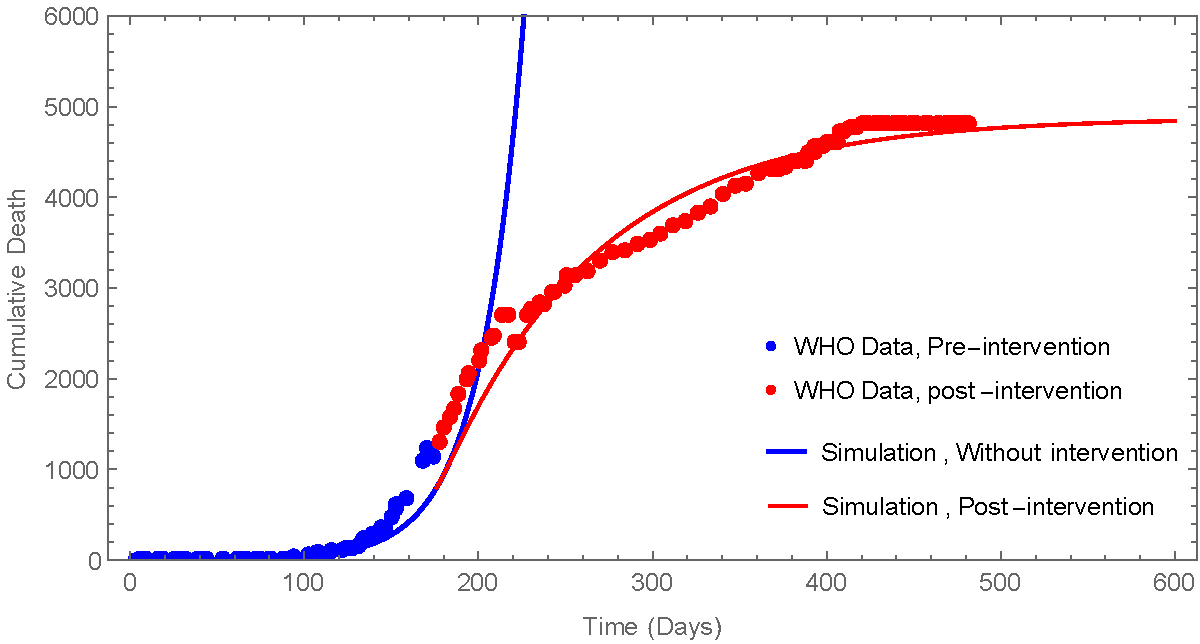
\includegraphics[width=1\textwidth]{ValidationPlot.pdf}
  \caption{Validation of calibration. Dots represent cumulative death data and the lines represent simulation based on mean posterior parameters. (Blue) - pre intervention and (red) - post treatment.}
\label{fig:Cumulative _Death}
\end{figure}






\subsection{Simulation}
 Insight Maker is a powerful online tool used to model and simulate complex systems. It utilizes different approaches, such as System Dynamics, Agent-Based Modeling and imperative programming. Insight Maker permits  construction of a graphical model to forecast the system response \cite{FortmannRoe}. We used the InsightMaker platform to prototype our model and simulate stepping forward through time. More details about the platform and its functionality can be found in Fortmann-Roe's review \cite{FortmannRoe}. The platform uses a fourth-order Runge-Kutta differential equation solver for the system dynamics model and  first order Euler approximation for the Agent-Based model.\\

\noindent The compartment S was initialized with a value of 999999, and the compartment I with 1, meaning that there is an infected individual per every million of individuals, the rest of the compartments were set to zero as an initial condition. The flow between the compartments is given in the equations and all the other parameters were initialized as shown in Table \ref{tab:parameters}.  As mention at the beggining of the section, the parameters were calibrated in two stages, before and after the international intervention. According with the time frame proposed, the change in the parameters was also implemented on Insight Maker. The links to the online models can be found on \cite{IM_AI} and  \cite{IM_BI}.  


% RESULTS AND DISCUSSION
%
%No intervention
\noindent After modeling the system with the parameters before the intervention, it can be observed in Figure \ref{fig:LB_IM_NoIn} how the total population decreases to 46.46\%  if there is no intervention and the each of the parameters continue to be the same. The number of susceptible individuals exponentially decays, converging to 7\% of the population, while exposed, infected, hospitalized and funeral comparments converges to zero; finally, after the system stabilizes, the final proportion of deaths would be 53.53\% 

\begin{figure}[!h]
  \centering
  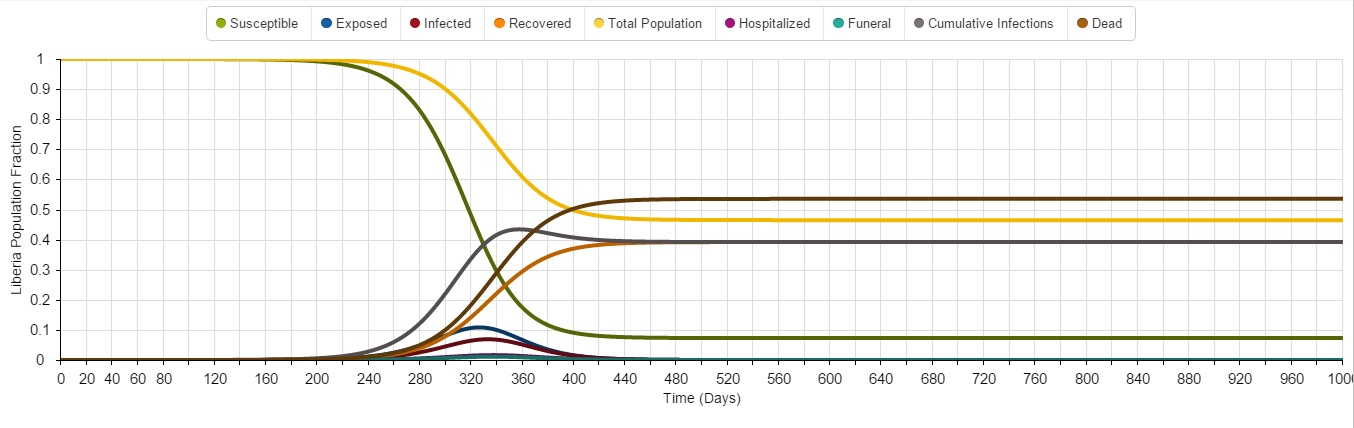
\includegraphics[width=1\textwidth]{LB_NoInt_SD_IM}
  \caption{Simulation results using the parameters of the first stage (Mar 2014  to Sept 2014) and assuming no intervention}
\label{fig:LB_IM_NoIn} 
\end{figure}

%Intervention 
\noindent As mentioned before, five parameters were calibrated for the second stage of the Ebola Outbreak, namely, community contact rate ($\beta_I$), hospital contact rate ($\beta_H$), funeral contact rate ($\beta_F$), time until hospitalization ($\gamma_H$) and probability a case is hospitalized ($\theta$). Figure \ref{fig:LB_IM_In} A. shows that there is not much change in the Total population and susceptible compartment, meaning that the virus was controlled;  Figure \ref{fig:LB_IM_In} B focuses on E, I, R, H , F and D compartments, showing that the international intervention causes a dramatic change in the behavior of such compartments.


\begin{figure}[h!]
 \centering 
 \begin{subfigure}[b]{1\textwidth}
  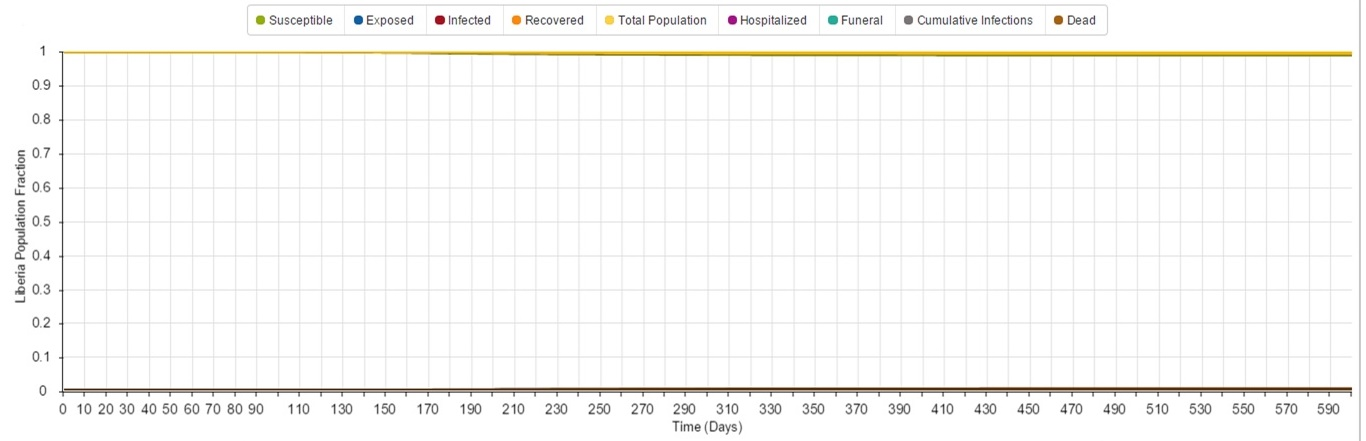
\includegraphics[width=\textwidth]{LB_Int3a_SD_IM} \caption{ Parameters of the first stage (March 2014  to Sept 2014)} \label{fig:LB_IM_In1} \end{subfigure}
 %
 \hspace{.1cm}
\begin{subfigure}[b]{1\textwidth}
 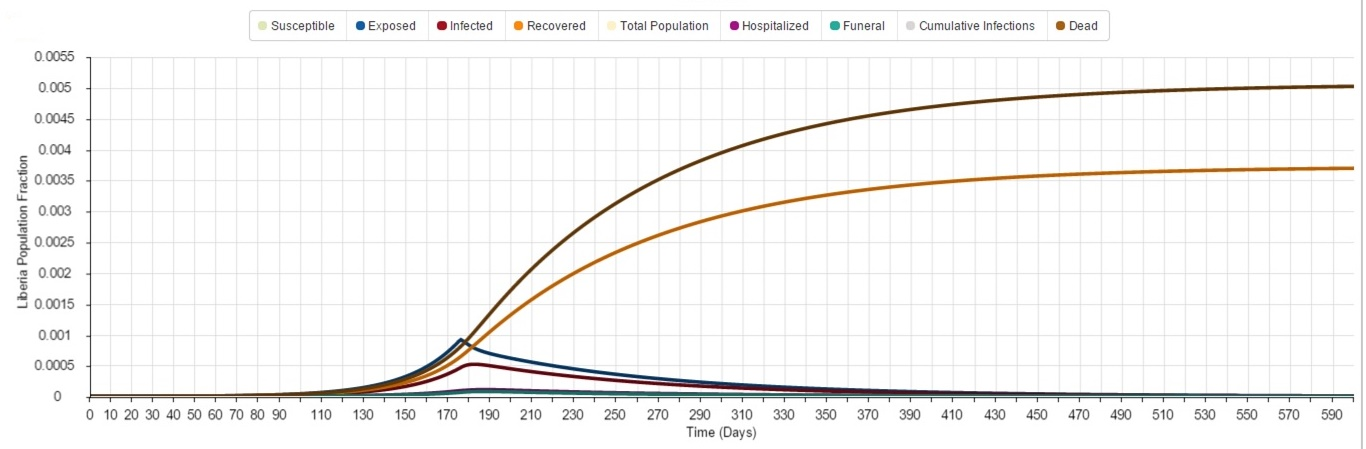
\includegraphics[width=\textwidth]{LB_Int3b_SD_IM} \caption{ Parameters of the second stage ( Sept 2014 to July 2015).} \label{fig:LB_IM_In2} \end{subfigure} \caption{Simulation Results}
\label{fig:LB_IM_In} 
\end{figure}





%Comparing with WHO data

\noindent Finally, a comparison between the proposed model and World Health Organization data is shown in Figures \ref{fig:LB_IM_WHO} and \ref{fig:LB_IM_WHO2}. As depicted in Figure \ref{fig:LB_IM_WHO}, there is a good fitting of our model with the data reported by WHO. Figure \ref{fig:LB_IM_WHO2} shows  the reported WHO data before and after intervention, the results of our model before and after intervention and the forecast for the coming months, predicting that after the system reaches an equilibrium, the proportion of deaths in Liberia product of the EVD would be 5.07\% approximately.



\begin{figure}[h!]
 \centering 
 \begin{subfigure}[b]{0.38\textwidth}
  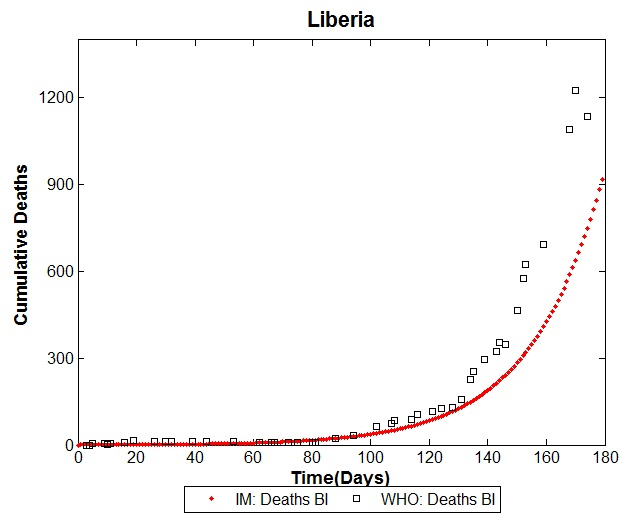
\includegraphics[width=\textwidth]{LB_BI_SD_WHO_IM} \caption{BI: Before Intervention Parameters (March 2014  to Sept 2014)} \label{fig:LB_BI_SD_WHO_IM} \end{subfigure}
 %
 \hspace{.1cm}
\begin{subfigure}[b]{0.38\textwidth}
 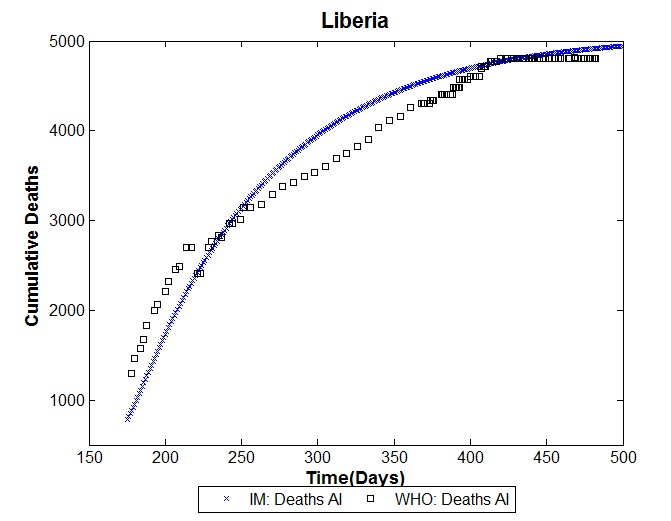
\includegraphics[width=\textwidth]{LB_AI_SD_WHO_IM} \caption{AI: After Intervention Parameters  ( Sept 2014 to July 2015).} \label{fig:LB_AI_SD_WHO_IM} \end{subfigure} 
\caption{Comparison between World Health Organization (WHO) data and Insight Maker (IM) results for cumulative deaths (D)}
\label{fig:LB_IM_WHO} 
\end{figure}



\begin{figure}[!h]
  \centering
  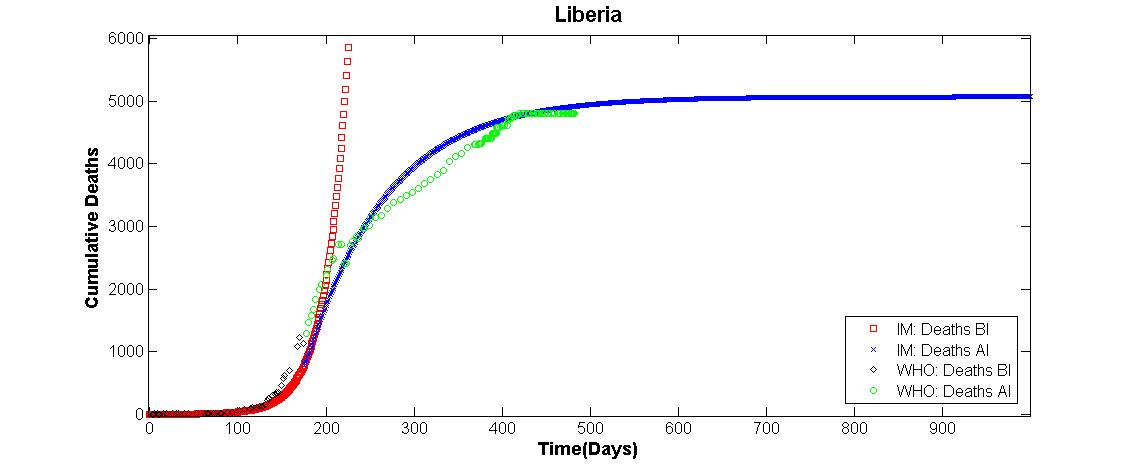
\includegraphics[width=1\textwidth]{LB_Int2_SD_WHO_IM}
  \caption{ Comparison between World Health Organization (WHO) data and Insight Maker (IM) results using the parameters before intervention (BI) and after intervention (AI), for the cumulative deaths (D).}
\label{fig:LB_IM_WHO2} 
\end{figure}


%%MATHEMATICA DESCRIPTION
Additionally, we drew the plots in the previous section also with Mathematica, and got almost same result. Furthermore, phase portraits of the system are shown in Figure \ref{fig:PhasePortrait}. 



\begin{figure}[h!]
 \centering 
 \begin{subfigure}[b]{0.38\textwidth}
  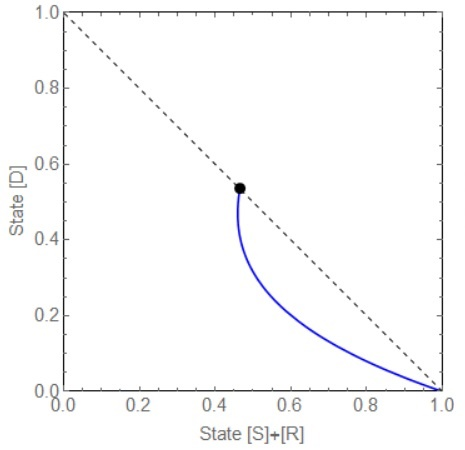
\includegraphics[width=\textwidth]{PhasePortraitA} \caption{NEED TO ADD)} \label{fig:PhasePortraitA} \end{subfigure}
 %
 \hspace{.1cm}
\begin{subfigure}[b]{0.38\textwidth}
 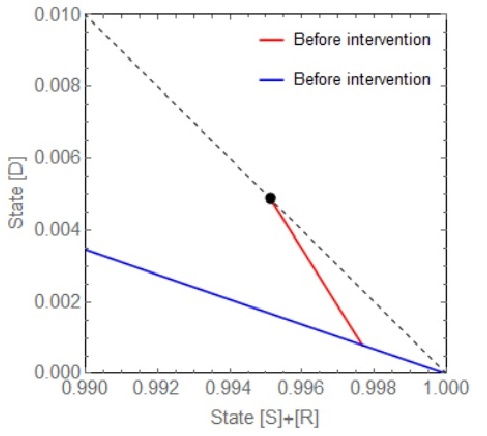
\includegraphics[width=\textwidth]{PhasePortraitB} \caption{NEED TO ADD).} \label{fiig:PhasePortraitB} \end{subfigure} 
\caption{Projection of phase portrait to (Susceptible + Recovered, Dead) space. (Blue) - without intervention, (Red) - with intervention, (Dots) - where the phase converges (equilibrium)}
\label{fig:PhasePortrait} 
\end{figure}





